\lab{The SVD and Image Compression}{SVD}

\objective{Learn how to compute the compact SVD. Explore the SVD as a method of matrix approximation, and use it to perform image compression.}
\label{lab:SVD}
% TODO
% - write a more compelling objective.
% - add references to the textbook and determine what is actually needed here. The explanation in the textbook is way better.
%


The \emph{Singular Value Decomposition} or \emph{SVD} is a matrix decomposition that is widely used in both theoretical and applied mathematics. 
Originally discovered by theoretical mathematicians, it is a canonical way to decompose a matrix.
Its practical use became apparent later on when Erhard Schmidt showed that the SVD could be a computational tool for providing low-rank matrix approximations.
Modern developments continue to confirm the importance of the SVD in both computational and theoretical applications.

\begin{comment}
The theoretical use of the \emph{Singular Value Decomposition} or \emph{SVD} has long been appreciated.
In fact, the idea of a canonical way of decomposing a matrix was so alluring that the SVD was independently discovered by at least four people through use of both  integral equations and systems of linear equations.

However, it wasn't until Erhard Schmidt showed how the SVD could be a computational tool for providing low-rank approximations that the practical applications became apparent.
Since Schmidt's work, further developments have confirmed the importance of the SVD in both computational and theoretical applications.
\end{comment}

\begin{comment}

The \emph{Singular Value Decomposition} is so important that it was discovered multiple times by different people in different ways.
The foundation work in systems of linear equations was laid by Gauss and Cauchy in the 1820's and later by Jacobi in 1846 with his work with the LU decomposition; however, the real work with the SVD started with Eugenio Beltrami.
In a paper he published in 1873 he was the first to work with the SVD; he was limited to real, square, nonsingular matrices with distinct singular values.
A year later, Camille Jordan published his own independent work that was more rigourus and avoided some of the pitfalls of Beltrami's research.
Together, Beltrami and Jordan are considered the codiscoverers of the singular value decomposition.

Later, James Joseph Sylvester independently presented an iterative algorithm and a rule for carrying out the reduction in 1889.
This rule was essentially Beltrami's work.
However Sylvester sent the note detailing his rule to the same journal Jordan had published in, showing not just his ignorance of Jordan's and Beltrami's works but his perception of the importance of the SVD.

The concurrent and independant derivation of the SVD shows its importance as a theoretical tool, but it wasn't until Erhard Schmidt discovered a computational use for the SVD that the practical applications became apparent.
Schmidt used integral equations rather than linear equations to derive the SVD, but
his most important contribution was showing how the SVD could be a computational tool to obtain optimal, low-rank approximations.

Since Schmidt's work, further devolpments have confirmed the importance of the SVD in both practical and theoretical applications.
\end{comment}

\subsection*{Computing the SVD}


The Singular Value Decomposition decomposes an $m \times n$ matrix $A$ into the form
\begin{equation*}
A = U \Sigma V^H
\end{equation*}
where $U$ and $V$ are square and unitary of sizes $m$ and $n$ respectively, and $\Sigma$ is diagonal and of size $m \times n$.
The values along the diagonal of $\Sigma$ are called the \emph{singular values} of $A$. 
These are also the square roots of the eigenvalues of $A^HA$.
% if $A$ is square, are equal to the absolute value of the eigenvalues of $A$.
Commonly the singular values are listed in decreasing order. Thus we have

\begin{equation*}
\Sigma = \mbox{diag}(\sigma_1,\sigma_2,\ldots,\sigma_n)
\end{equation*}
where $\sigma_1 \geq \sigma_2 \geq \ldots \geq \sigma_n \geq 0$ are the singular values of $A$.

If A is of rank $r$, then A has exactly $r$ nonzero singular values.
The first $r$ columns of U span the range of A, and the last $n -r$ columns span the null space of $A^H$.
Likewise, the first $r$ columns of V span the range of $A^H$ and the last $m - r$ span the null space of $A$.

For a more in-depth definition and proof that the SVD exists for every matrix, refer to the book (TODO: ref textbook) .
Here we will focus on computing the SVD. 

First, we define two modifications of the regular SVD.
In the \emph{compact SVD}, we only keep the $r$ nonzero singular values.
Only $r$ column vectors of $U$ and $r$ row vectors of $V^H$, corresponding to the $r$ singular values, are calculated.
The compact SVD takes the form $A= U_r \Sigma_r V_r^H$ where $U_r$ is $m\times r$, $\Sigma_r$ is $r\times r$ and diagonal, and $V_r^H$ is $r\times n$.
Although we drop the decompositions of the nullspaces, by calculating $U_1 \Sigma_1 V_1^H$ we can still recover the full matrix $A$.

The \emph{truncated SVD} is similar to the compact SVD, but instead of keeping all the nonzero singular values, we only keep the $k$ largest.
While this saves space, it means that we cannot recover the whole matrix.
Instead we end up with $\widehat A_k = U_k\Sigma_k V_k^H$ where $\widehat A_k$ is a rank $k$ approximation of $A$, $U_k$ is $m\times k$, $\Sigma$ is $k \times k$ and diagonal, and $V_k^H$ is $k \times n$.

The components of the compact or truncated SVD can be calculated as follows:
\begin{itemize}
\item The singular values of $A$, which form the diagonal of $\Sigma$, are the square roots of the eigenvalues of $A^HA$. 
These are sorted in descending order. 
For the compact SVD, keep all of the nonzero singular values. 
For the truncated SVD, keep only the largest $k$.
\item The columns of $V$ are the eigenvectors of $A^HA$, where the $i$th column $V_i$ matches the $i$th singular value.
\item The columns of $U$ are $U_i = \frac{1}{\sigma_i} AV_i$.
\end{itemize}

\begin{comment}
\begin{algorithm}
\begin{algorithmic}[1]
\caption{SVD for Full Rank Square Matrices.}
\label{Alg:svd_full}
\Procedure{SVD}{$A$}
\State $n \gets \shape{A}$
\State $eigs \gets$ eigenvalues$(A^HA)$
\State sort$(eigs)$
\State $V \gets$ eigenvectors$(A^HA)$
\State $svals \gets \sqrt{eigs}$
\State $U \gets \allocate{n,n}$
\For{$i=0\ldots n-1$}
      \State $U_i \gets  \frac{1}{svals[i]} AV_i$
\EndFor
\State $S \gets$ diag$(svals)$
\State \pseudoli{return} $U, S, V^H$
\EndProcedure
\end{algorithmic}
\end{algorithm}
\end{comment}

\begin{problem}
Write a function \li{truncated_svd} that accepts a matrix $A$ and an optional integer \li{k = None}. 
If \li{k} is \li{None}, calculate the compact SVD. If \li{k} is an integer, calculate the truncated SVD.
(Note: if there are fewer than \li{k} nonzero singular values, the truncated SVD will come out the same as the compact SVD.)
Since the only difference between these two processes is the number of singular values we keep, we only need to write one function.

\begin{enumerate}
\item Find the eigenvalues and eigenvectors of $A^H A$.
\item Find the singular values of $A$. Keep only the greatest \li{k}, and discard any that are equal to zero.
\item Calculate $V$.
\item Calculate $U$.
\end{enumerate}

Return U, the diagonal of $\Sigma$, and V.
Check your function by calculating the compact SVD and seeing if $U\Sigma V^H = A$ using \li{np.allclose()}.

Hint: When calculating the SVD, you will need to sort the eigenvalues while keeping track of their associated eigenvectors. 
Consider the function \li{np.argsort} for keeping the eigenvalues and eigenvectors in the same order while sorting.
%Look for places to use fancy indexing when sorting and selecting the singular values.
\label{prob:calc_svd}
\end{problem}

\begin{comment}
%Commented out because finding the rest of the SVD isn't important to this lab.
%They can reference the book for this information.
If $A$ is full rank and square, it has $n$ nonzero singular values and this process gives us the full SVD.
If $A$ is not full rank or not square, we can compute the first $r$ columns of $U$ and $V$, where $r$ is the number of nonzero singular values, in this way.
To find the rest of the SVD, we can use Gram-Schmidt orthonormalization.

More specifically, let $r$ be the number of nonzero singular values.
If $r<n$ then we only have $r$ eigenvectors to fill $V$, which is a $n\times n$ matrix.
We find the remaining columns of $V$ by using Gram-Schmidt orthonormalization to finish the basis for $n$-space.
Similarly, if $r<m$ then we only have $r$ columns of $U$ so we use Gram-Schmidt orthonormalization to finish the basis for $m$-space.
The compact SVD does not have this problem because $U_1$ and $V_1$ only have $r$ columns, the remaining columns are the decomposition of the null space of the matrix, and are not included.
In this lab we calculate the compact SVD for simplicity.
\end{comment}

\begin{info}
In practice, calculating $A^HA$ in order to find its eigenvalues is unstable.
We use this method here because it is mathematically the simplest.
Industrial SVD solvers, however, use different methods that avoid computing $A^HA$.
\end{info}

\subsection*{Visualizing the SVD}
Recall that a matrix is one way to express a linear transformation.
An $m\times n$ matrix defines a linear transformation that sends points from $\mathbb{R}^n$ to $\mathbb{R}^m$.

Intuitively, the SVD can be thought of as breaking a linear transformation into more basic steps.
The SVD decomposes a given matrix into two rotations and a scaling.
$V^H$ represents a rotation, $\Sigma$ represents a rescaling along the principal axes, and $U$ represents another rotation.


\begin{figure}
\centering
\begin{subfigure}[b]{.49\textwidth}
  \centering
  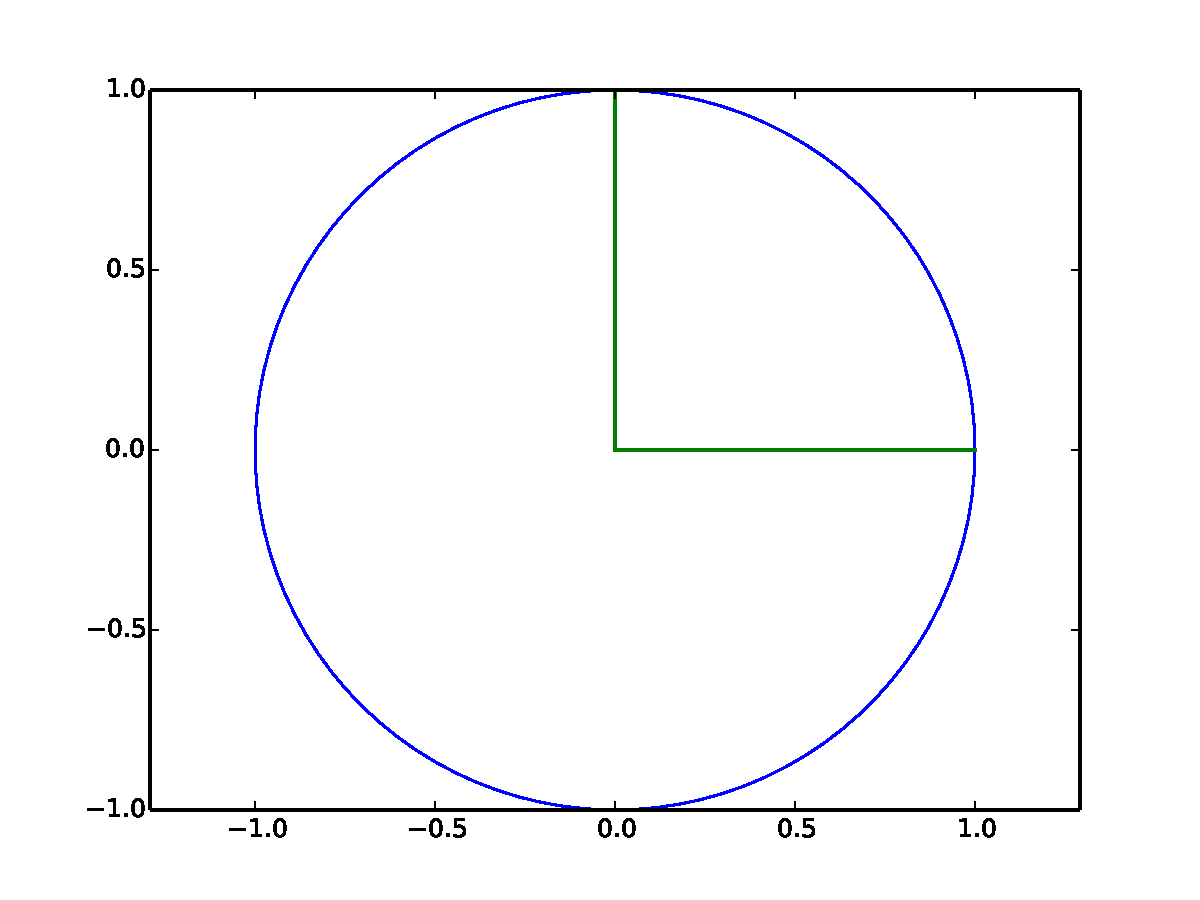
\includegraphics[width=\textwidth]{unit_circle.pdf}
  \caption{The unit circle, $S$, with two unit vectors.}
\end{subfigure}
\begin{subfigure}[b]{.49\textwidth}
  \centering
  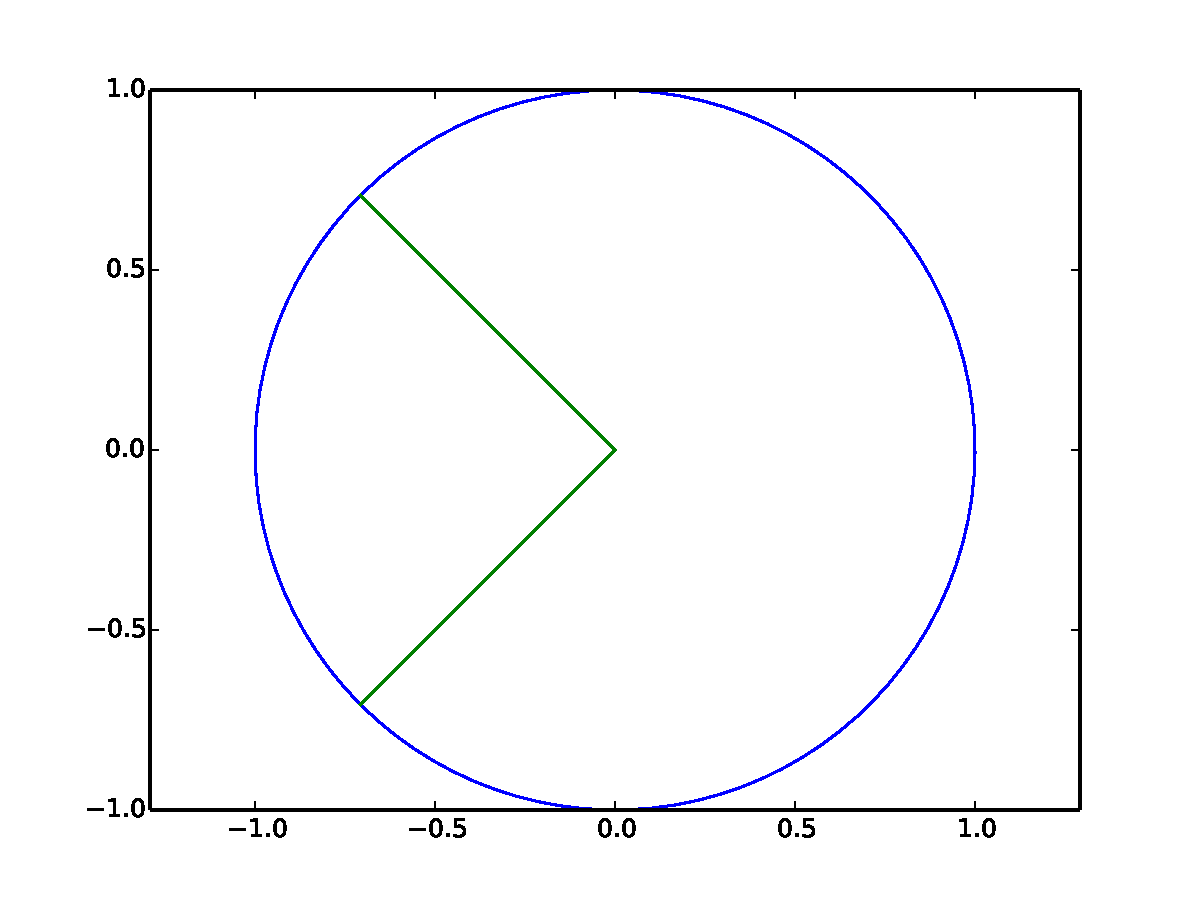
\includegraphics[width=\textwidth]{vcircle.pdf}
  \caption{$V^HS$}
  %\label{fig:svals_plot}
\end{subfigure}
\begin{subfigure}[b]{.49\textwidth}
  \centering
  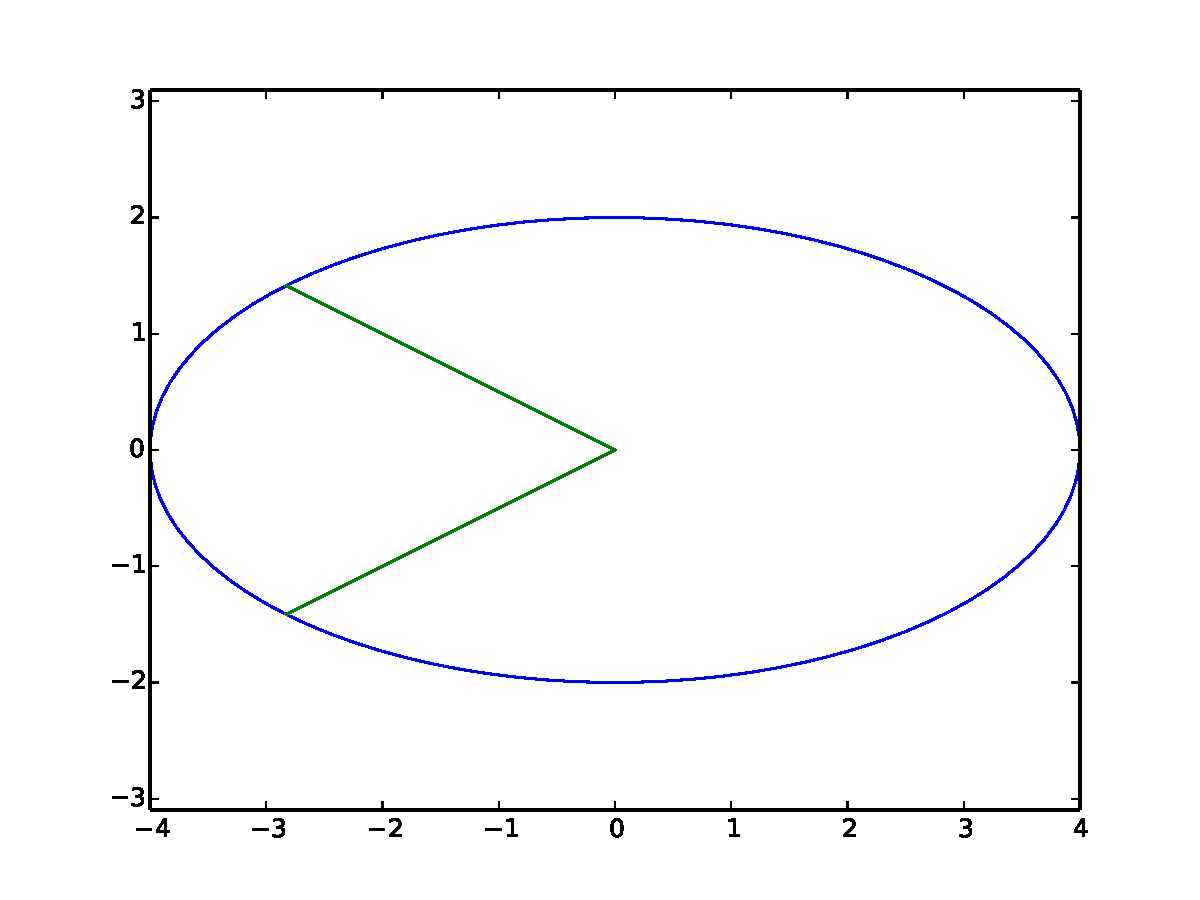
\includegraphics[width=\textwidth]{svcircle.pdf}
  \caption{$\Sigma V^H S$}
  %\label{fig:svals_plot}
\end{subfigure}
\begin{subfigure}[b]{.49\textwidth}
  \centering
  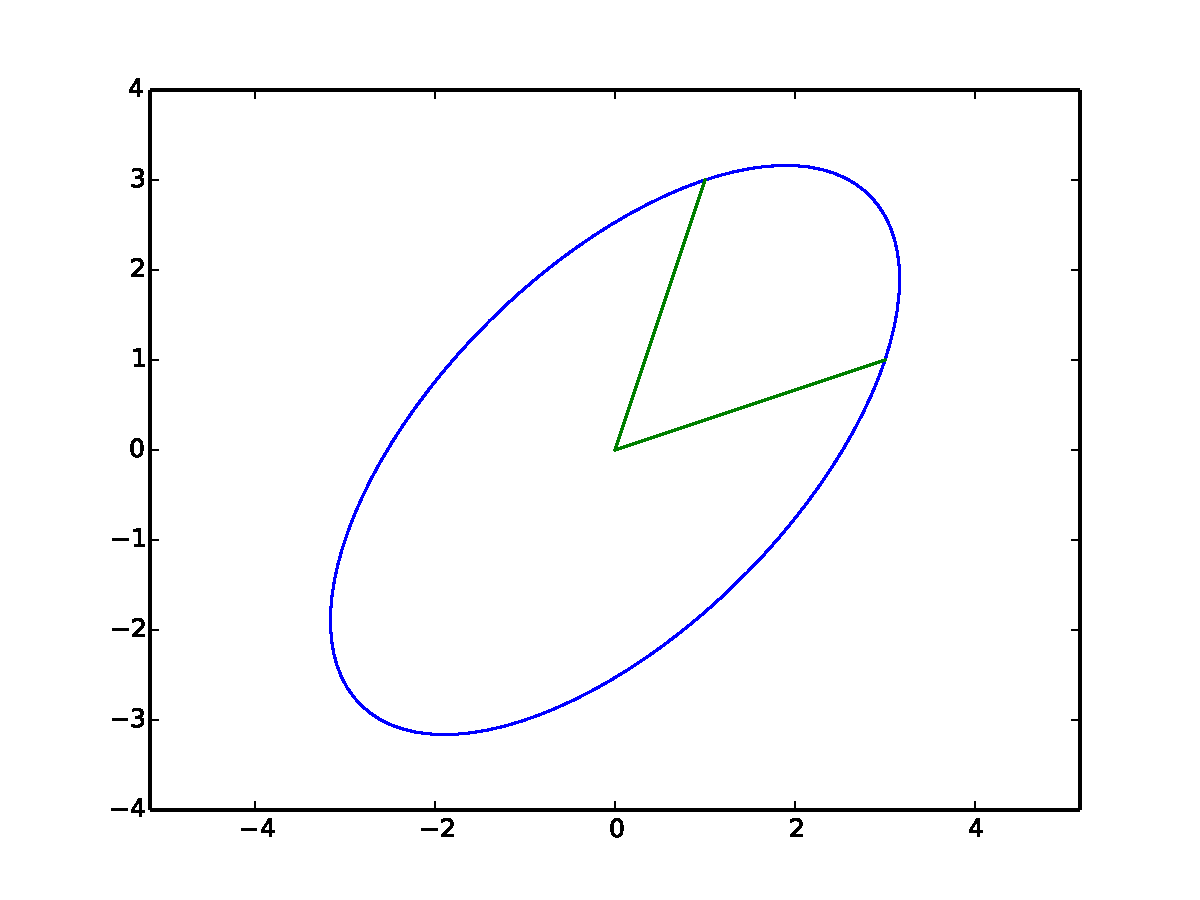
\includegraphics[width=\textwidth]{full_transformation.pdf}
  \caption{$U \Sigma V^H S$}
  %\label{fig:svals_plot}
\end{subfigure}
\caption{Each step in transforming the unit circle and two unit vectors using the matrix $A$.}
\label{fig:sol1}
\end{figure}

\begin{problem}
In this problem we will use the SVD to visualize how the matrix
\begin{equation}
A =  \begin{pmatrix}3 & 1\\1 & 3\end{pmatrix}
\end{equation}
acts on points in $\mathbb{R}^2$.
Given a set of points $S$ in $\mathbb{R}^2$, we can calculate the transformation $AS$ in steps by using the SVD $A = U\Sigma V^H$.

Show the steps of the transformation of $S$ in four separate subplots.
Plot $S$ first to show the untransformed points.
To visualize the steps of the transformation, plot the points $V^HS$, then $\Sigma V^HS$, and finally $U\Sigma V^HS$.
Your solution should look like Figure \ref{fig:sol1}.

Use the set of points $S$ stored in the \li{circle.npz} dataset.
This dataset contains a set of points on the unit circle and a set of unit vectors. 
You can access the circle by loading the \li{"circle"} file. 
You can access the unit vectors by loading the \li{"unit_vectors"} file. 
These points are stored as a numpy array of points in $\mathbb{R}^2$ with the first row being all the x-coordinates and the second row being all the y-coordinates.
\end{problem}

\begin{comment}
\subsection*{Image Data Compression}
In this lab, we explore how the SVD can be used to compress image data.
Recall that an image is simply a matrix where each position is the color value for the pixel in that position.
The SVD lets us choose how much information to keep, and what information is most important.
Larger eigenvalues correspond to columns of $U$ and $V$ that contain more information, while smaller eigenvalues correspond to less important columns.
This idea is used in many areas of applied mathematics including signal processing, statistics, semantic indexing (search engines), and control theory.
\end{comment}

\subsection*{The SVD and Data Compression}
We now turn to computational uses of the SVD. We will explore how the SVD is useful for matrix approximations, and use it to compress images.

\subsection*{Low-Rank Matrix Approximation}
If the rank $r$ of a matrix $A$ is significantly smaller than its dimensions, the compact SVD offers a way to store $A$ with less memory.
Without the SVD, an $m\times n$ matrix requires storing $mn$ values.
By decomposing the original matrix into the compact SVD, $U_r$, $\Sigma_r$ and $V_r$ together require $mr+r+nr$ values.
This is an efficient storage method if $r$ is much smaller than both $m$ and $n$.
For example, suppose $m=100$, $n=200$ and $r=20$.
Then the original matrix would require storing $20,000$ values whereas the compact SVD only requires storing $6020$ values.

The truncated SVD allows even greater efficiency.
By only keeping the first $k$ singular values, we can create an approximation $\widehat A_k = U_k\Sigma_k V_k^H$.
This requires storing only $mk+k+nk$ values.
As we make $k$ small, we eventually require very little storage---but at the cost of losing information from the original matrix.

The beauty of the SVD is that it keeps the information that is most important. 
Larger singular values correspond to columns of $U$ and $V$ that contain more information, and so dropping the smallest singular values retains as much information as possible.
When approximating a matrix at a lower rank, the truncated SVD is guaranteed to give the closest approximation possible.
In mathematical terms, given a matrix $A$ and its SVD approximation $\widehat A_k = U_k\Sigma_k V_k^H$, the matrix $\widehat A_k$ is the \emph{best rank $k$ approximation} to $A$ (with respect to the induced 2-norm and Frobenius norm). TODO: ref textbook.

This is a significant and ubiquitous concept, appearing in areas including signal processing, statistics, semantic indexing, and control theory.


\begin{comment}
We can also calculate $\widehat A$ by finding the full SVD, and setting all singular values after the $k$th to zero.
Thus the modified $\Sigma$ would be
\begin{equation*}
\Sigma_{\widehat A} = \mbox{diag}(\sigma_1,\sigma_2,\ldots,\sigma_s,0,\ldots,0).
\end{equation*}
Multiplying this matrix with the original $U$ and $V^H$ will give the same $\widehat A$ that was found by computing the truncated SVD directly.
\end{comment}


To create lower-rank approximations in practice, we can use SciPy's linear algebra module, which has a convenient method to calculate the SVD of a given matrix. 
The code below computes the SVD of \li{A}.
\begin{lstlisting}
>>> import numpy as np
>>> import scipy.linalg as la
>>> A = np.array([[1,1,3,4], [5,4,3,7], [9,10,10,12], [13,14,15,16], [17,18,19,20]])
>>> U,s,Vh = la.svd(A, full_matrices=False)
\end{lstlisting}
In the last line of code, we included the keyword argument \li{full_matrices=False} to calculate the
compact SVD rather than the full SVD. The arrays \li{U} and \li{Vh} correspond to the matrices
$U_r$ and $V_r^H$ discussed earlier. The array \li{s} gives the nonzero singular values
of the matrix \li{A}, and we can find the rank of \li{A} by inspecting the number of entries in \li{s} (here we have a rank 4 matrix). 

Next, we calculate a rank 3 approximation.
We take the first three singular values, first three columns of \li{U}, and first three rows of \li{Vh}.
We omit the last singular value from the calculation along with the last column of \li{U} and last row of \li{Vh}.

\begin{lstlisting}
>>> S = np.diag(s[:3])
>>> Ahat = U[:,:3].dot(S).dot(Vh[:3,:])
>>> la.norm(A-Ahat)
\end{lstlisting}
Note that $\widehat A$ is ``close'' to the original matrix $A$, but that its rank is 3 instead of 4. 

\begin{problem}
Write a function \li{svd_approx} that takes as input a matrix $A$ and a positive integer $k$ and returns 
the best rank $k$ approximation to $A$ (with respect to the induced 2-norm and Frobenius norm).
Use \li{scipy.linalg.svd}.
\label{prob:svd_approx}
\end{problem}

Recall that the error between the best rank $s$ approximation $\widehat{A_s}$ to $A$ with respect to the induced 
2-norm is given by
$$
\|A - \widehat{A_s}\|_2 = \sigma_{s+1},
$$
where $\sigma_{s+1}$ is the $(s+1)$-th singular value of $A$. 
TODO: ref textbook.

This offers a way to approximate a matrix subject to an error tolerance: 
choose the truncated SVD approximation such that the largest discarded singular value is less than the error tolerance.

\begin{problem}
Using \li{scipy.linalg.svd}, write a function \li{lowest_rank_approx} that takes as input a matrix $A$ and a positive number $e$ and returns
the lowest rank approximation of $A$ with error less than $e$ (with respect to the induced 2-norm).
You should only calculate the SVD once.
\end{problem}


\begin{comment}
The reduced form of the SVD also provides a way to approximate a matrix with another one of lower rank.
This idea is used in many areas of applied mathematics including signal processing, statistics, semantic indexing (search engines), and control theory.
If we are given a matrix $A$ of rank $r$, we can find an approximate matrix $\widehat A$ of rank $s<r$ by taking the SVD of $A$ and setting all of its singular values after $\sigma_s$ to zero, that is,
\begin{equation*}
\Sigma_{s} = \mbox{diag}(\sigma_1,\sigma_2,\ldots,\sigma_s,0,\ldots,0)
\end{equation*}
and then multiplying the matrix back together again.
The more singular values we keep, the closer our approximation is to $A$.
The number of singular values we decide to preserve depends on how close of an approximation we need and what our size requirements are for $U_1$, $\Sigma_{\widehat A}$, and $V_1$.
Try plotting the singular values.
\end{comment}

\subsection*{Application to Image Compression}

Sometimes there is not enough available bandwidth to transmit a full resolution photograph.
Suppose you need to transmit an image from a remote location.
You might aim to reduce the amount of data being sent, while also minimizing the loss of detail in the image.

This can be done using the SVD.
An image is just a matrix of pixel values, which means it has a singular value decomposition.
Computing and sending a low-rank SVD approximation of the image can considerably reduce the amount of data sent, while retaining a high level of image detail.

Examining the singular values of an image gives an idea of how low-rank the approximation can be.
Figure \ref{fig:hubble} presents an image and a log plot of its singular values from greatest to least.
The plot in \ref{fig:svals_plot} is typical of a photographic image;
the singular values start out large but drop off rapidly.
In this rank $670$ image, $624$ of the singular values are $50$ or more times smaller than the largest singular value.
By discarding these relatively small singular values, we can retain nearly all of the image detail, while storing only a rank 46 image!
This is a huge reduction in data size.

Figure \ref{fig:rankvalues} shows several low-rank approximations of the image in Figure \ref{fig:hubble_original}.
Even at a very low rank the image is recognizable.
By rank 40, the approximation visibly differs very little from the original.

\begin{figure}
\centering
\begin{subfigure}[b]{.49\textwidth}
\centering
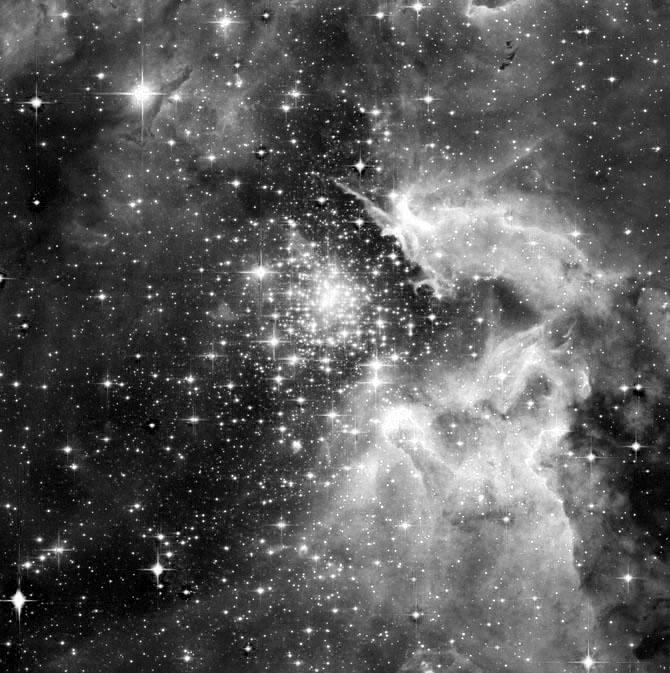
\includegraphics[width=\textwidth*5/6]{hubble_red}
\caption{NGC 3603 (Hubble Space Telescope).}
\label{fig:hubble_original}
\end{subfigure}
\begin{subfigure}[b]{.49\textwidth}
\centering
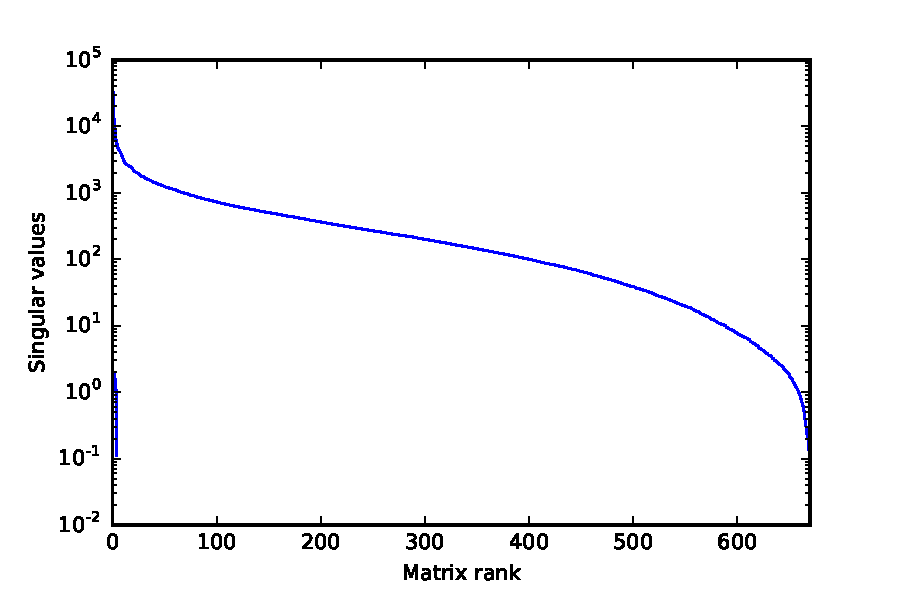
\includegraphics[width=\textwidth*5/4]{hubble_svals}
\caption{Singular values from greatest to smallest on a log scale}
\label{fig:svals_plot}
\end{subfigure}
\caption{An image and its singular values.}
\label{fig:hubble}
\end{figure}

\begin{figure}
\centering
\begin{subfigure}[b]{.35\textwidth}
\centering

\includegraphics[width=\textwidth]{rank1.jpg}
\caption{Rank 1}
\end{subfigure}
\begin{subfigure}[b]{.35\textwidth}
\centering
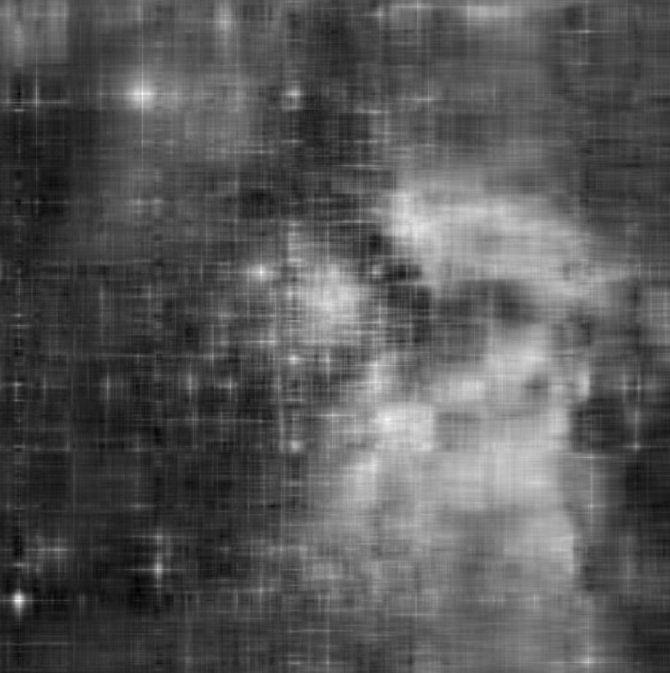
\includegraphics[width=\textwidth]{rank14.jpg}
\caption{Rank 14}
\end{subfigure}

\begin{subfigure}[b]{.35\textwidth}
\centering
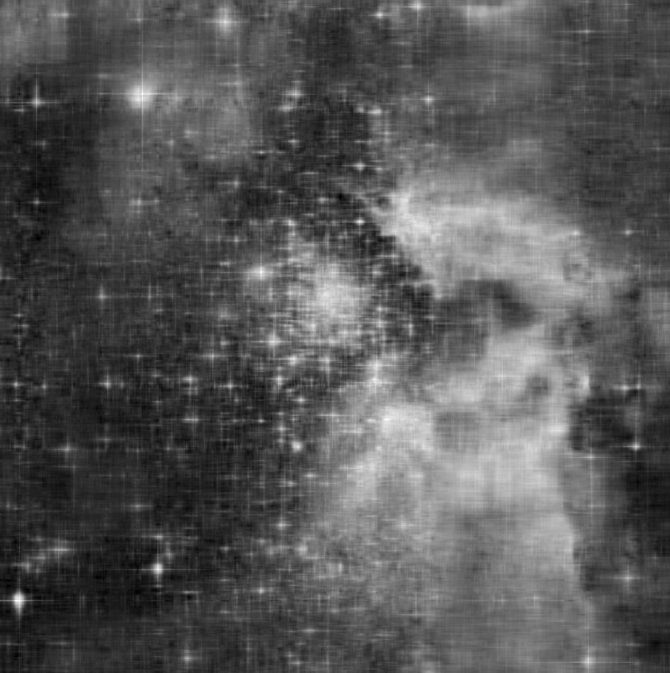
\includegraphics[width=\textwidth]{rank27.jpg}
\caption{Rank 27}
\end{subfigure}
\begin{subfigure}[b]{.35\textwidth}
\centering
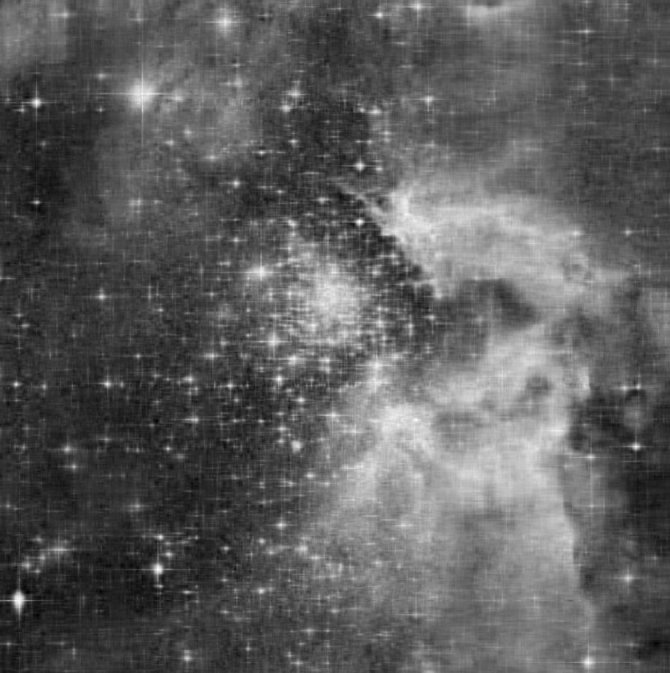
\includegraphics[width=\textwidth]{rank40.jpg}
\caption{Rank 40}
\end{subfigure}
\caption{Different rank approximations for SVD-based compression.  Notice that higher rank is needed to resolve finer detail.}
\label{fig:rankvalues}
\end{figure}

The code below reads in an image, converts it to black and white, and shows it.
The function from Problem \ref{prob:svd_approx} can then be used to calculate an approximation of \li{X}.
%Enter the following into IPython (note that any image you might have will work):
\begin{lstlisting}
>>> import matplotlib.pyplot as plt
>>> # Take only one layer (layer 0) of the image
>>> X = plt.imread('hubble_image.jpg')[:,:,0].astype(float)
>>> X.nbytes     #number of bytes needed to store X
>>> plt.imshow(X, cmap="gray")
>>> plt.show()
\end{lstlisting}
\begin{comment}
Computing the SVD of your image is simple.
Remember to make the singular values a diagonal matrix before multiplying.
\begin{lstlisting}
>>> U,s,Vt = svd(X, full_matrices=False)
>>> S = sp.diag(s)
\end{lstlisting}
In the next code block, $k$ represents the desired rank of the output.
\begin{lstlisting}
>>> k = 50
>>> u1, s1, vt1 = U[:,0:n], S[0:n,0:n], Vt[0:n,:]
>>> Xhat = u1.dot(s1).dot(vt1)
>>> (u1.nbytes + np.diag(s1).nbytes + vt1.nbytes) - X.nbytes   #should be negative
>>> plt.imshow(Xhat)
>>> plt.show()
\end{lstlisting}
\end{comment}

\begin{problem}
Using the \li{svd_approx} function from Problem \ref{prob:svd_approx}, write a function \li{compress_img} that accepts two parameters \li{filename} and \li{k}. The function should plot the original image and the best rank k approximation of the original image. 

While \li{svd_approx} worked for grayscale images, the \li{compress_img} function should work on color images. 
You may split the image into its three RGB layers and approximate each layer separately, then recombine them.
Your output should be similar to Figure \ref{fig:compressed_image}.

Hints:
\begin{itemize}
\item Sometimes \li{plt.imshow} does not behave as expected when being passed RGB values between 0 and 255. It behaves much better when being passed values between 0 and 1. 
\item Since the SVD provides an approximation, it is possible that the SVD will generate values slightly outside the valid range of RGB values. 
To fix this, use fancy indexing (as discussed in the NumPy and SciPy lab) to set values greater than 1 to 1 and values less than 0 to 0. 
\end{itemize}

\begin{figure}[H]
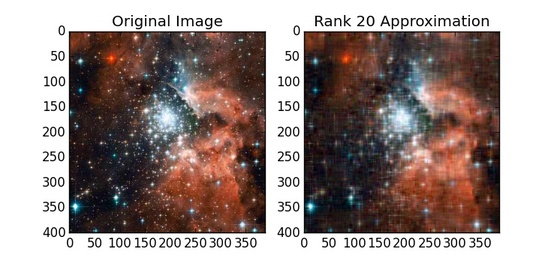
\includegraphics[width=\textwidth]{compressed.jpg}
\caption{Correct output for the best rank 20 approximation.}
\label{fig:compressed_image}
\end{figure}
\end{problem}
